\tikzset{every picture/.style={line width=0.75pt}} %set default line width to 0.75pt        

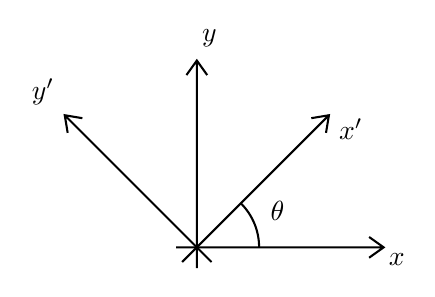
\begin{tikzpicture}[x=0.75pt,y=0.75pt,yscale=-1,xscale=1]
%uncomment if require: \path (0,300); %set diagram left start at 0, and has height of 300

%Shape: Axis 2D [id:dp6052588153202806] 
\draw  (214,173) -- (314,173)(224,83) -- (224,183) (307,168) -- (314,173) -- (307,178) (219,90) -- (224,83) -- (229,90)  ;
%Shape: Axis 2D [id:dp2386863255816345] 
\draw  (216.93,180.07) -- (287.64,109.36)(160.36,109.36) -- (231.07,180.07) (279.15,110.77) -- (287.64,109.36) -- (286.23,117.85) (161.77,117.85) -- (160.36,109.36) -- (168.85,110.77)  ;
%Shape: Arc [id:dp02254630738242136] 
\draw  [draw opacity=0] (245.21,151.79) .. controls (245.21,151.79) and (245.21,151.79) .. (245.21,151.79) .. controls (245.21,151.79) and (245.21,151.79) .. (245.21,151.79) .. controls (251.07,157.64) and (254,165.32) .. (254,173) -- (224,173) -- cycle ; \draw   (245.21,151.79) .. controls (245.21,151.79) and (245.21,151.79) .. (245.21,151.79) .. controls (245.21,151.79) and (245.21,151.79) .. (245.21,151.79) .. controls (251.07,157.64) and (254,165.32) .. (254,173) ;  

% Text Node
\draw (225,78) node [anchor=south west] [inner sep=0.75pt]    {$y$};
% Text Node
\draw (315,174.4) node [anchor=north west][inner sep=0.75pt]    {$x$};
% Text Node
\draw (291,109.4) node [anchor=north west][inner sep=0.75pt]    {$x'$};
% Text Node
\draw (143,90.4) node [anchor=north west][inner sep=0.75pt]    {$y'$};
% Text Node
\draw (258,149.4) node [anchor=north west][inner sep=0.75pt]    {$\theta $};


\end{tikzpicture}
